
\chapter{Fuels}
\section{Introduction}
	Fuels have an influence on the engine design, the torque, consumption, reliability, ... There exists solid, liquid and gaseous fuels, the liquid one being the most used. 
	
\subsection{Requirements}
	\begin{itemize}
	\item[•] High combustion value, more energy, when transport we can store it in a much smaller liter because there are more energy. In the batteries, the energy value is smaller than in fuel for example. For a car it is important but for an industrial use, we don't care. \\
	
	\item[•] It has to be easely and efficiently producible, small carbon footprint. it is easier to produce oil than coal for example.\\
	
	\item[•] The start and end of the combustion should be controllable, spark or compression. In some fuel we cannot control the start of combustion, like in CI engine where the fuel burn by compression.\\
	
	\item[•] Transport is important for vehicles. Diesel is much more safe than petrol for example. Alternative fuel like hydrogen, to store and use it we have a lot of safety issues, much more difficult. \\
	
	\item[•] A lot of emissions, main focus today is to reduce the emissions. $CO_2$ is causing a global climate change, depending on the fuel it will produce more (diesel) or less (petrol) $CO_2$. We try to have minimum impact on the environment.\\
	
	\item[•] Life cycle as low as possible. 
	\end{itemize}
	
\section{Liquid fuels}
	\textbf{Crude oil} is a mixture of hydrocarbons. The oil has a specific density that decreases with the processes, it depends also on the quality of the oil (depending on the region). First phase, we go over a distillation, the lighter components goes to the top of the distillation tower and the heavier are below. It is easier to sell lighter fuels than the heavier.
	We take the sulfur out because it is polluting, negative effects: oxidation $\rightarrow$ sulfur oxide, in the air causes acid rains. Second effect, in compression ignition engine, it stimulates the formation of soude, it is why it is more and more reduced in the fuel. \\
	
Type of fuel: at the top of the distillation tower we have \textbf{gas} like methane (important greenhouse gas), ethane (LPG) and propane (compressed natural gas). 
Then petrol and gasoline (spark ignition engine). Kerosene (tractors, airplanes, ...)
Gasoil and diesel (compression ignition engine). Heavy fuel (home burners, heavy fuel, high viscosity, we can heat it up and then inject it). Lubrification oil and
asphalt are the the one at the very lower part of the distillation. 

In fact, all the fuels are mixture of hydrocarbons with different structures and molecular mass. For example, the fuel used in winter and in summer is not the same, they are adjusted to get the best properties. 

\wrapfig{12}{l}{8.5}{0.3}{ch3/1}{fig:3.1}
Here we can see the places in the world where we can find oil. Most fuel are found in Africa, South America and Mexico, United States. Some of the countries has less sulfur in the oil than the others. The oil naps are found by stating gravitational changes in the ground. They introduce some pressure in the ground to exploit the oil. Notice that today we also have ships where the distillation process is executed. Petroleum gas can be used in LPG or in the combustion of the distillation tower. 

\subsubsection{Hydrocarbons}	
	\wrapfig{15}{r}{8.5}{0.3}{ch3/2}{fig:3.2}	
	Normal paraffines, isoparaffines, olefines, … If you look to the oxidation reaction, some will react very easily with air, others not. Benzene (\textbf{aromatics}) for example resists throw oxidation, it complicates the combustion, this is an advantage to control the combustion (spark ignition for example), but can be undesirable for diesel (compression). Aromatics are undesirable because it is cancerous, so we try to not use it in fuel. \textbf{Isoparaffines} combust very well in contact of air. \textbf{Making a fuel is mixing hydrocarbons} to get a good combination, if the environment and the condition changes, we have to adapt our composition. For example, in winter the fuel is lighter to make it evaporate during combustion, in summer we have to make it heavier to not evaporate it too rapidly. 
	
\subsection{Characteristics}
\subsubsection{Petrol (gasoline)}
	Fuels are standardized, it is different from the USA to Europe. The boiling traject (30\degres C - 200\degres C) indicates how easy the fuel evaporates, we have a range of temperature to respect. The composition is also standardized: 60-80\% paraffines, 15-30\% naftenes, 0-10\% aromatics, 0-2\% olefines. \textbf{Octane number} is the most important characteristic for petrol. Density is limited, so the fuel is lighter than water (0.72-0.775 kg/l).
	
\subsubsection{Diesel (gasoil)} 
In diesel we have less aromatics (because it is resistant to evaporation) and more paraffines (easy auto ignition), boiling traject indicates that the fuel is heavier (180\degres C - 370\degres C). The most important number for diesel is Cetane number. For fast running engines (cars) this varies between 45 and 55 while for slow ones it is more than 30 (ships). The density is higher than gasoline but still less than water (0.82-0.86 kg/l).

\section{Fuel criteria (petrol)}
\subsection{Parameters}
	Petrol is the first fuel we are studying, spark ignition engine can have 4 or 2 strokes, we have to mix the fuel with oil in the 2 strokes case, but we discuss only the petrol used without oil. 
	
	\begin{center}
	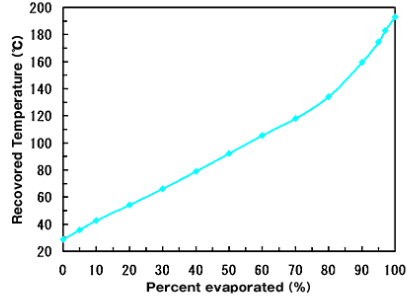
\includegraphics[scale=1]{ch3/3}
	\captionof{figure}{}
	\label{fig:3.3}
	\end{center}
	
	\begin{itemize}
	\item[•] In a spark ignition engine we will mix air and fuel before injection, we should get a precise state before combustion. The important is that when the fuel air mixture is in the cylinder, the fuel must evaporate in the air. At the end of the compression stroke, we want the fuel to be completely evaporated. This is the criterion of \textbf{volatility}. The testings are done in lab. For a good cold engine start, we can have 10\% of the liquid evaporated and in hot engine 90\% (avoids condensation and lubrification oil dilution). If the fuel is too volatile, we will get vapor locks in the fuel supply. Indeed, the fuel is pumped. This process creates heat and if the fuel is volatile, we can have an underpressure at the inlet of the pump, that will block the machinery (\autoref{fig:3.3}). \\
	
	\item[•] Vapour pressure is the pressure above the fuel itself. We limit it to 60kPa in summer and in winter 90kPa in winter. In summer the fuel is heavier, so it starts to boil at a higher temperature, while in winter it is the contrary. This is why we should have less vapour pressure for summer.\\
	
	\item[•] Vaporization heat: the vaporization needs heat, so the temperature of all other mixtures will decrease. In the air we have water, if the temperature goes down too much we will have icing for example. The 3 last parameters are the criteria before combustion. \\
	
	\item[•] Auto-ignition temperature: we want to control the ignition with the spark. But auto-ignition happens without control, we want to avoid that. So that temperature will be higher for petrol (480-550\degres C, 1 Atm) than diesel (330-350\degres C, 1 Atm).
	\end{itemize}
	
\subsection{Deflagration and detonation}	
	\wrapfig{12}{l}{8}{0.25}{ch3/4}{fig:3.4}	
	Before the compbustion, we have an inlet of air/fuel mixture, which is then compressed and then burned. The normal combustion is the \textbf{deflagration}, we have the spark that ignite the fuel in the neighborhood of the spark, if all the condition are good, we start burning, the surrounding fuel mixture will start warming up and then burning and the rest follow. We have some flame going layer per layer, until the progression of the flame front fill the entire combustion chamber. The speed of the flame front is \textbf{subsonic}! \\
	
\wrapfig{12}{r}{8}{0.25}{ch3/5}{fig:3.5}	
\textbf{Detonation} is operated at much higher pressure and much higher speed of flame front. We get the same beginning, the flame front moves, but due to pressure buildup, deposits, … the far field \textbf{auto-ignites}! This is supersonic and goes faster than deflagration. The detonation produces explosions of high pressures that will slow down the piston in its moving, causing vibrations. It can destroy the engine because of the local pressure and large heat production. How can we avoid that? The base parameter is the fuel, so we have to control this process by the fuel. We can see on the figure that the pressure in the combustion chamber normally evolves as a sine, but when there are detonations, this is disturbed. 

\subsubsection{Fuel criteria}
\begin{itemize}
\item[•] Fuel is very difficult to ignite and burn if it has not the right mixture of air and fuel. The limits are 1-6.9\% of petrol in air. This is performed in a carburetor.\\

\item[•] \textbf{Octane number} is the most important number for avoiding auto ignition. If we use a fuel with only iso-octane $C_8H_{18}$, that fuel is 100\% knock free. On the other hand, if we had a fuel composed only of normal heptane  $C_7H_{14}$, we would always have knocks. That is why the Octane number is 0 for normal heptane and 100 for iso-octane. When knock was detected long time ago, they wanted to adapt the fuel to avoid detonation. And the American society said let's make a reference engine and let's do the test on that testing engine (\textbf{CFR}), they are still used today. It has never been modified. We canmake some parameters vary to study the fuel. On base of the compression ratio we can calculate the octane number. \\

We have different kind of Octane numbers: Research Octane Number (RON) which is for normal use in a car, the MON (Engine Octane Number) is used in the USA, the difference can go up to 15, and the last is the Road Octane Number (RdON) which is the one measured in road conditions. \\

\item[•] How do we get a high Octane Number? The main parameter is the hydrocarbon structures, branched, short, unsaturated, cyclic. We can also add some oxygeneous components like alcohols, but the volatility increase can damage the material. 
\end{itemize}

\section{Combustion in diesel engines}
	\wrapfig{10}{l}{6}{0.3}{ch3/6}{fig:3.6}	
	Here is represented the evolution of the pressure in the combustion chamber when combustion happens and when not. We see that we go to much higher temperatures and higher pressures when combustion. The injector injects small drops of fuel into the hot air already in the chamber, compressed. In the ideal case, we would like the fuel to burn immediately when injected, but it is not the case, we have an \textbf{ignition lag}. 
	
	\ \\
	
\begin{center}
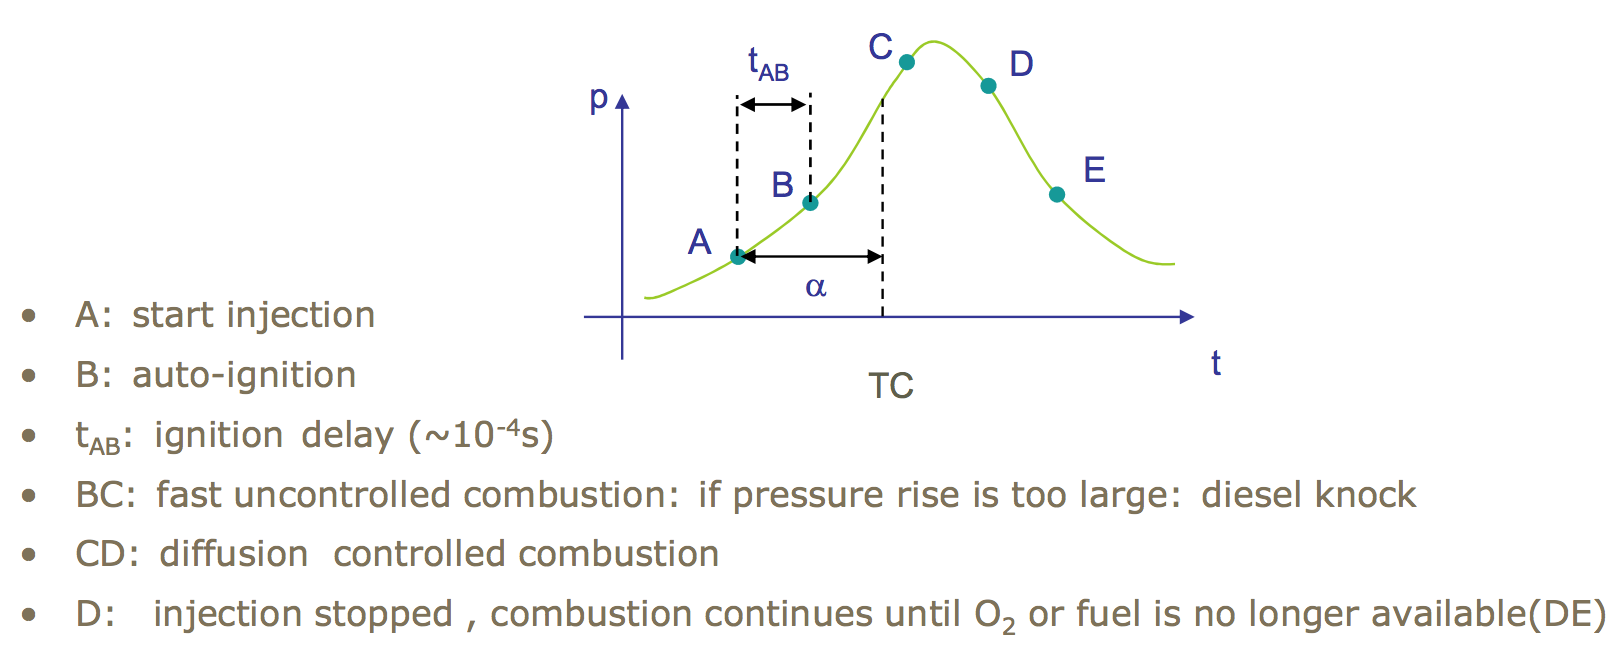
\includegraphics[scale=0.45]{ch3/7}
\captionof{figure}{}
\end{center}

We can also have diesel knocks. These ones are influenced by: 
	\begin{itemize}
	\item[•] The pre-ignition angle, which is today fully controlled electronically, it influences the amount of fuel injected. Pre-injection consist in injecting a few drops, then waiting it to burn and then doing the main injection. We avoid the knock where too much drop burn together and introduces a high amount of sudden energy. 
	
	\item[•] The ignition delay is very important because if it's high, the combustion will only start when the piston is already going down. Today, we control that completely electronically.
	
	\item[•] If the air is too cold and the pressure too low, it will take too much time to burn the fuel. When the fuel starts to burn, it causes a sudden increase in energy and pressure so diesel knock (vibration). It will not arm the engine directly, because the engine is fitted for high pressures and the knock disappear in a certain time. To avoid this, we warm the engine, heat up the air.
	\end{itemize}
 
\subsection{Parameters}
	\begin{itemize}
	\item[•] You can imagine that \textbf{volatility} is not the main issue of the diesel engine because we inject drops directly in hot air, the large volatility is not required. \textbf{Flashing point} is the point of temperature where we can ignite the vapor above the liquid (>55\degres C). The \textbf{viscosity }is more important than petrol, when we will inject it we will have to apply much higher power. \\
	
	\item[•] Deposits and corrosion are a big problem for diesel engines, we spoke about sulfur, this one is a bigger problem in diesel fuel because it is more heavy. It also causes soude emissions, dangerous for health. \\
	
	\item[•] The ignition delay is as we said the delay between injection and ignition. This can be decreased by increasing the compression ratio, the inlet pressure and temperature. The larger are these values, the closer the auto-ignition conditions are reached after compression. The Cetane number gives information about that. \\
	
	\item[•] Diesel knocks manifest as a too large and fast pressure rise before TC. This can be due to too early pre-injection or too high injection flow rate. \\
	
	\item[•] The Cetane number is the percentage of cetane ($C_{16}H_{34}$) in a mixture of cetane and alpha methylnaphtaline ($C_{11}H_{10}$) that has the same ignition delay as the examined fuel. High Cetane number states good auto-ignition. It is also measured on a CFR engine but diesel. For fast running engines this should be about 50-55, and for slow running engines about 30-35. Low Cetane number means that the fuel favorises the formation of knocks, high pressure and temperature and increased NOX emission, but means thermal stability. While for high Cetane number this means that the fuel has a high proportion of paraffines that are unstable. \\
	
	\item[•] Good starting properties: we have to make sure that the boiling point is low enough to get auto-ignition. Cold resistancy: when temperatures are low, the paraffin cristalizes and can block the filters. To avoid this, we have heated filters. 
	\end{itemize}		
	
	
\section{Alternative fuels}
	\begin{center}
	\begin{minipage}{0.4\textwidth}
	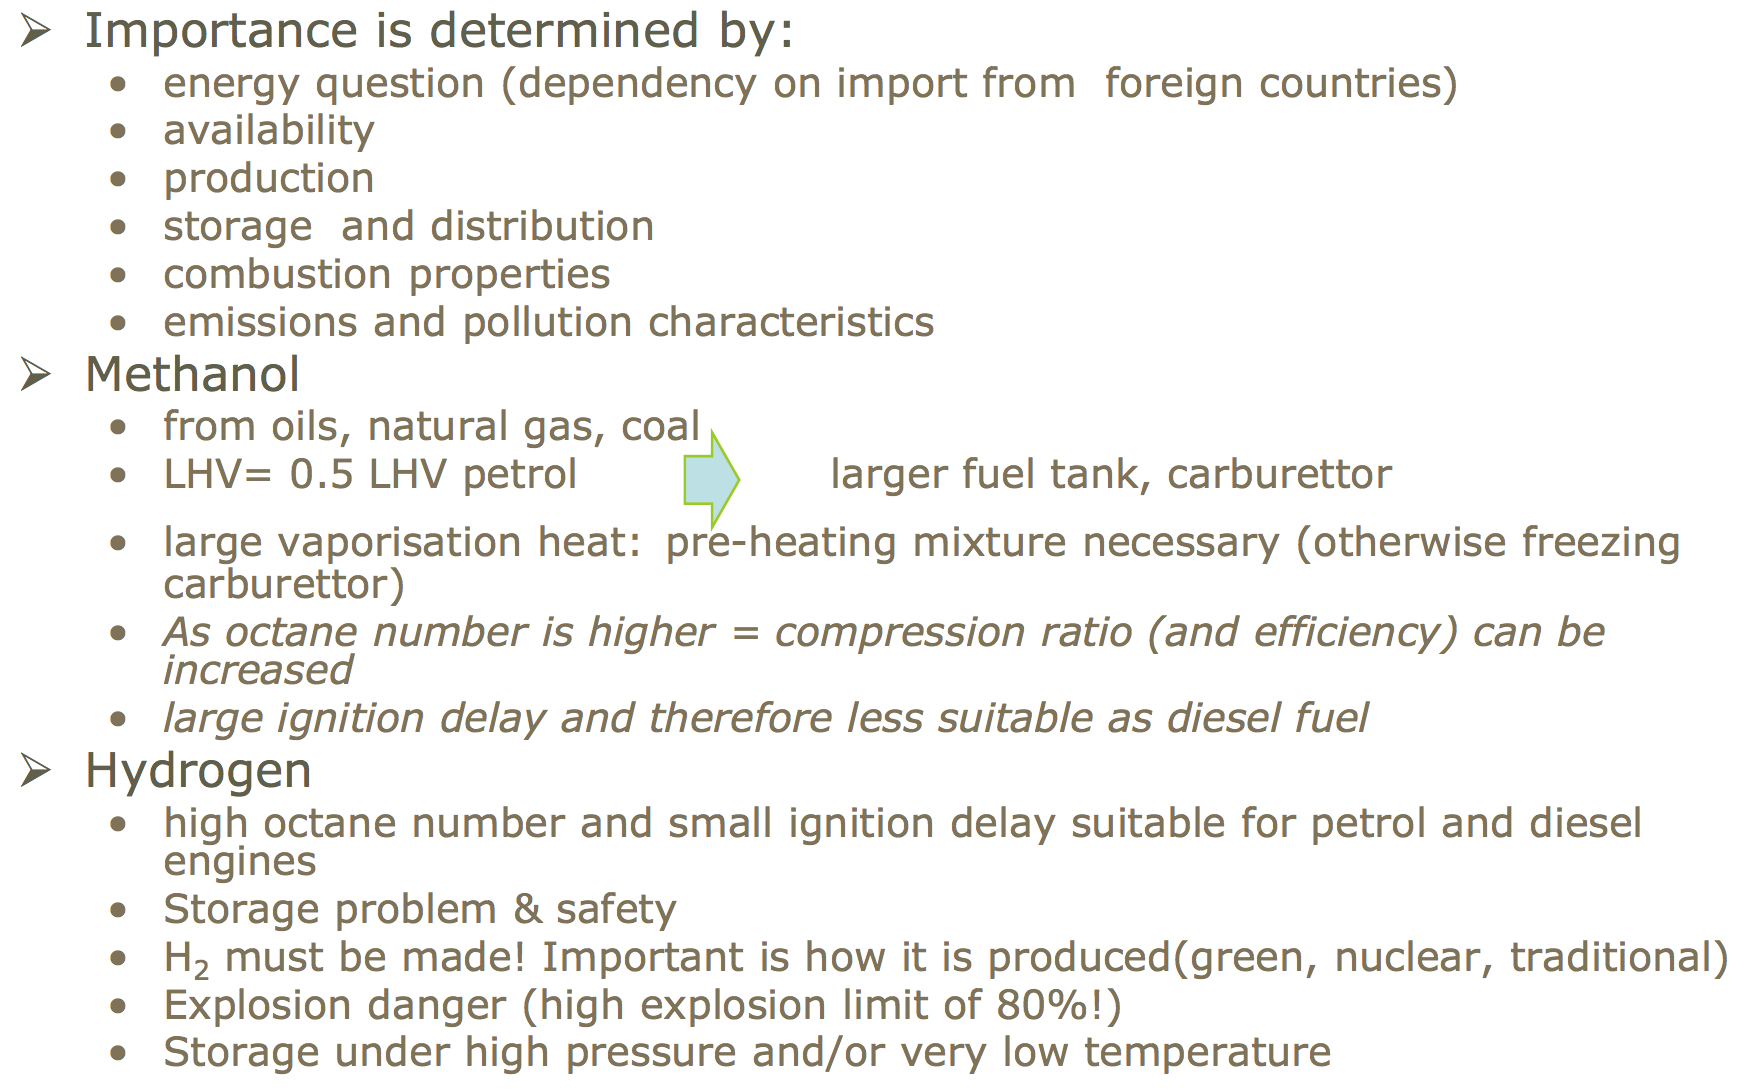
\includegraphics[scale=0.3]{ch3/8}
	\captionof{figure}{}
	\end{minipage}
		\begin{minipage}{0.5\textwidth}
	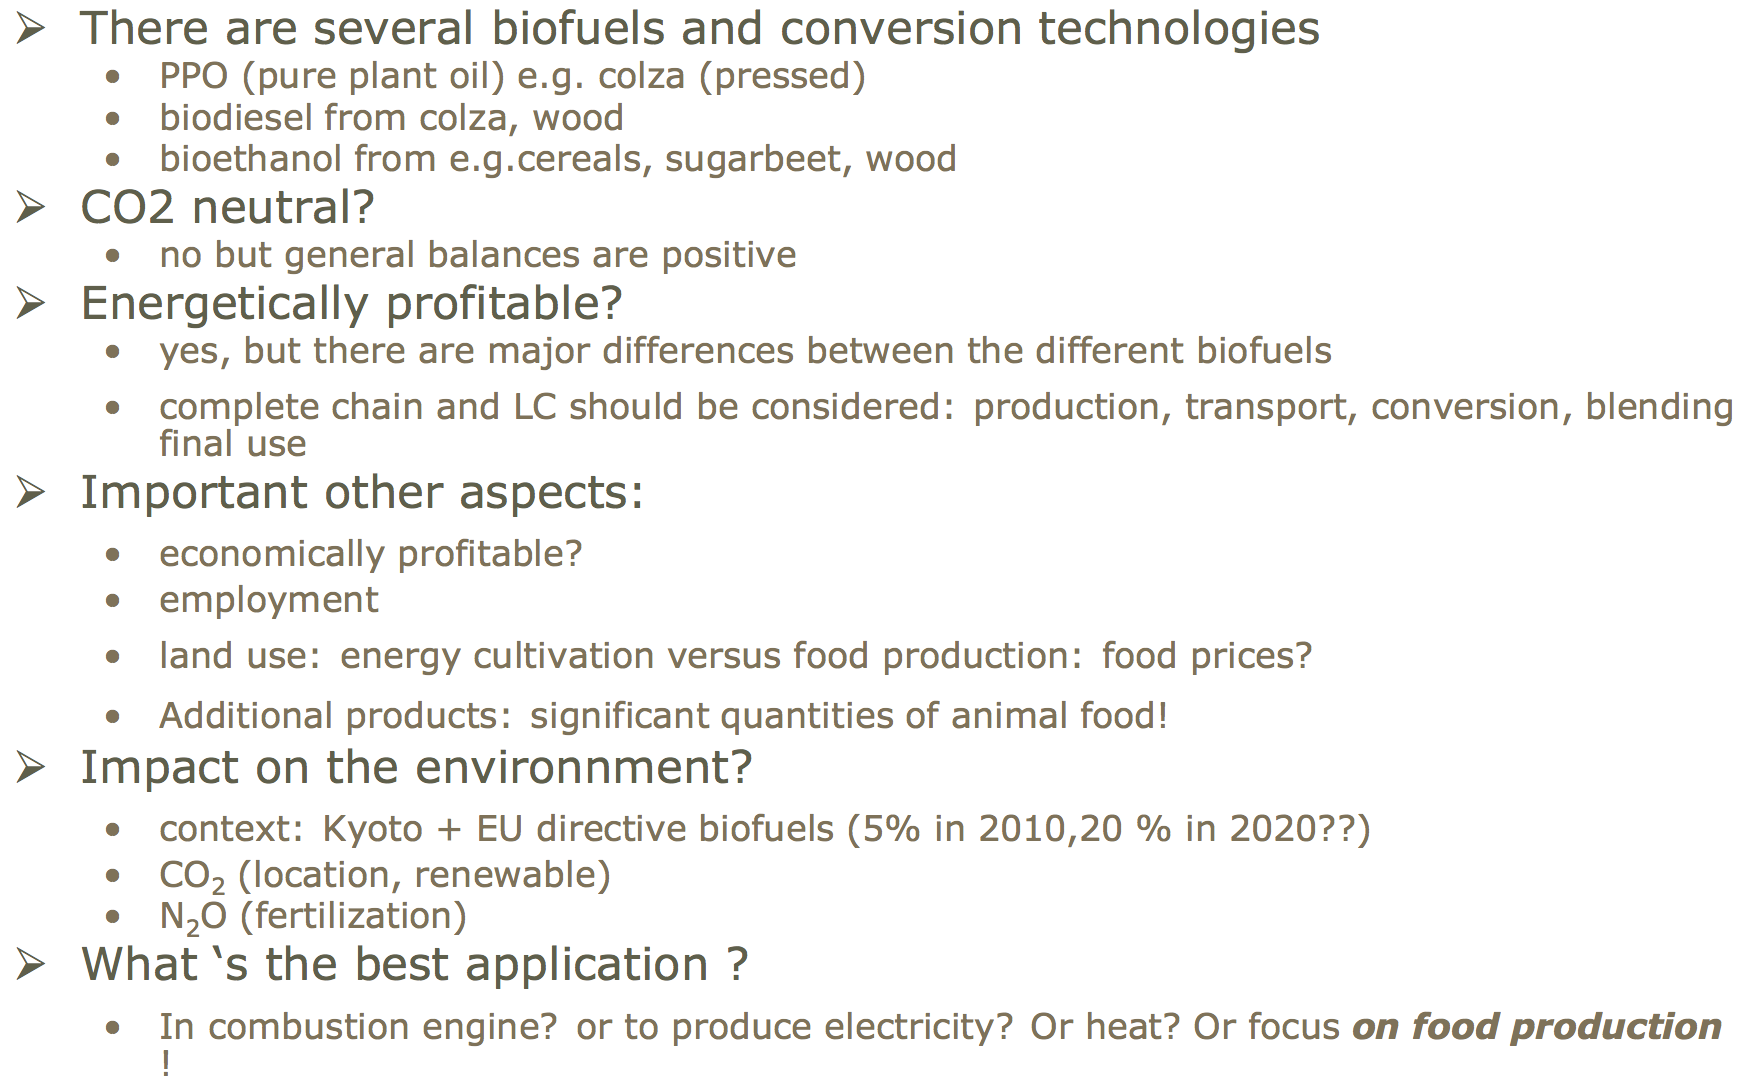
\includegraphics[scale=0.3]{ch3/9}
	\captionof{figure}{}
	\end{minipage}
	\end{center}














